\subsection{Abordagem gulosa}

    Algoritmo guloso é a estratégia que tenta resolver o problema fazendo a 
    escolha localmente ótima em cada fase com a esperança de encontrar 
    uma ótima global que resolve o problema por completo.

    Na solução de alguns problemas combinatórios a estratégia gulosa pode
    assegurar a obtenção de soluções ótimas, o que não é muito comum. No
    entanto, quando o problema a ser resolvido pertencer à classe NP-completo
    ou NP-difícil, a estratégia gulosa torna-se atrativa para a obtenção de
    solução aproximada em tempo polinomial.

    Um exemplo de abordagem gulosa é o Algoritmo de Dijkstra.

\subsubsection{Algoritmo de Dijkstra}

    \begin{figure}[ht]
        \centering
        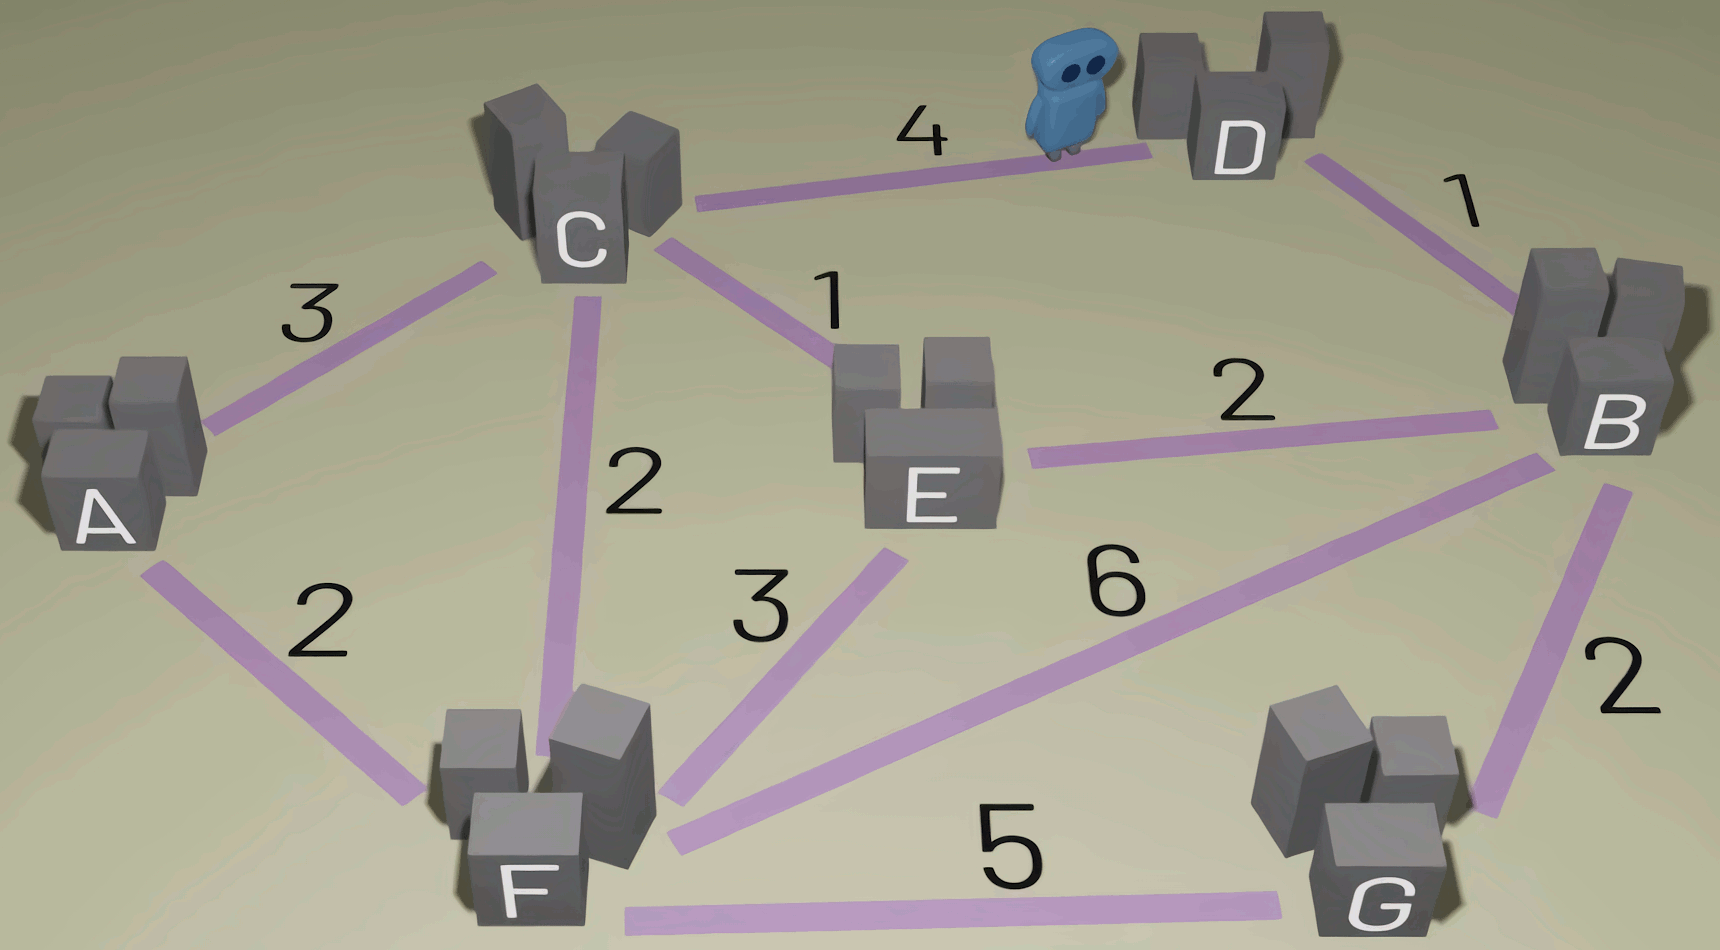
\includegraphics[width=.7\textwidth]{dijkstra.png}
        \caption{Encontrar menor caminho}
        \label{fig:dikstra}
    \end{figure}

    Dado um grafo qualquer, e dois pontos: partida e chegada, encontre o menor caminho possível.
    Para resolver esse problema, Dijkstra cria o que é chamado de \emph{Shortest path tree}(spt) ou 
    a árvore de caminho mais curto. A cada passo do algoritmo a \textbf{spt} adiciona uma vértice não visitada,
    e então atualiza a distância das adjacências da vértice que foi adicionada. O algoritmo irá terminar, quando 
    a \textbf{spt} conter informação de todas as vértices.

    \newpage 

    \begin{algorithm}
        \caption{Dijkstra} 
        \begin{algorithmic}[1]
        \Procedure{Dijkstra}{origin,destination}
        \For{$\text{each v $\in$ G.vertices}$}
        \State {$\text{distance[v] = $\infty$}$}
        \EndFor
        \State {$\text{A $\leftarrow$ G.vertices}$}
        \State {$\text{distance[origin] = 0}$}
        \For{$\text{j = 1 in $\mid G.vertices\mid$ -1}$}
        \State {$\text{u := Extract-Min(A)}$}
        \State {$\text{A.pop(u)}$}
        \For{$\text{each v $\in$ Neighbors(u)}$}
        \State {$\text{Update(distance,v)}$}
        \EndFor
        \EndFor
        \State {$\text{\textbf{return} distance[destination]}$}
        \EndProcedure
        \end{algorithmic}
    \end{algorithm}

    \subsubsection{Algoritmo Guloso Vs Backtracking}

    \begin{itemize}
        \item Ambos tentam procurar pela solução ótima global, e tem casos
        onde isso é possível, porém, há casos que o algoritmo encontra a solução 
        sub-optimizada
        \item Devido a natureza da estratégia de backtracking, tais algoritmos costumam ter 
        implementações recursivas, enquanto que algoritmos gulosos tentam 
        buscar a melhor escolha local de forma iterativa.
    \end{itemize}

    \subsubsection{Algoritmo Guloso Vs Branch-and-Bound}

    \begin{itemize}
        \item Ambos tentam procurar pela solução ótima global, e tem casos
        onde isso é possível, porém, há casos que o algoritmo encontra a solução 
        sub-optimizada
        \item Devido a natureza da estratégia de backtracking, tais algoritmos costumam ter 
        implementações recursivas, enquanto que algoritmos gulosos tentam 
        buscar a melhor escolha local de forma iterativa.
    \end{itemize}

    \nocite{greedy-algorithm}

\newpage